\begin{frame}[label=p28_20260920]{\strut}
\centering\vfill
\makebox[\textwidth][c]{%
\begin{beamercolorbox}[wd=0.68\textwidth,sep=1.2em,center,rounded=true,shadow=true]{block body}
{\LARGE\bfseries Thanks for listening!}\par\vspace{1em}
{\large Reporter: Lekai Yao}\par\vspace{0.45em}
{\large 2026.9.20}
\end{beamercolorbox}}
\vfill
\end{frame}

\appendix
\setbeamertemplate{footline}{\hfill\usebeamercolor[fg]{structure}\small Backup\quad\insertframenumber\hspace{0.4cm}\vspace{0.15cm}}
\begin{frame}[label=p29_20260920]{Backup: 7v17 fit at xeff 40\%}
\begin{columns}[c]
\column{0.65\textwidth}\centering
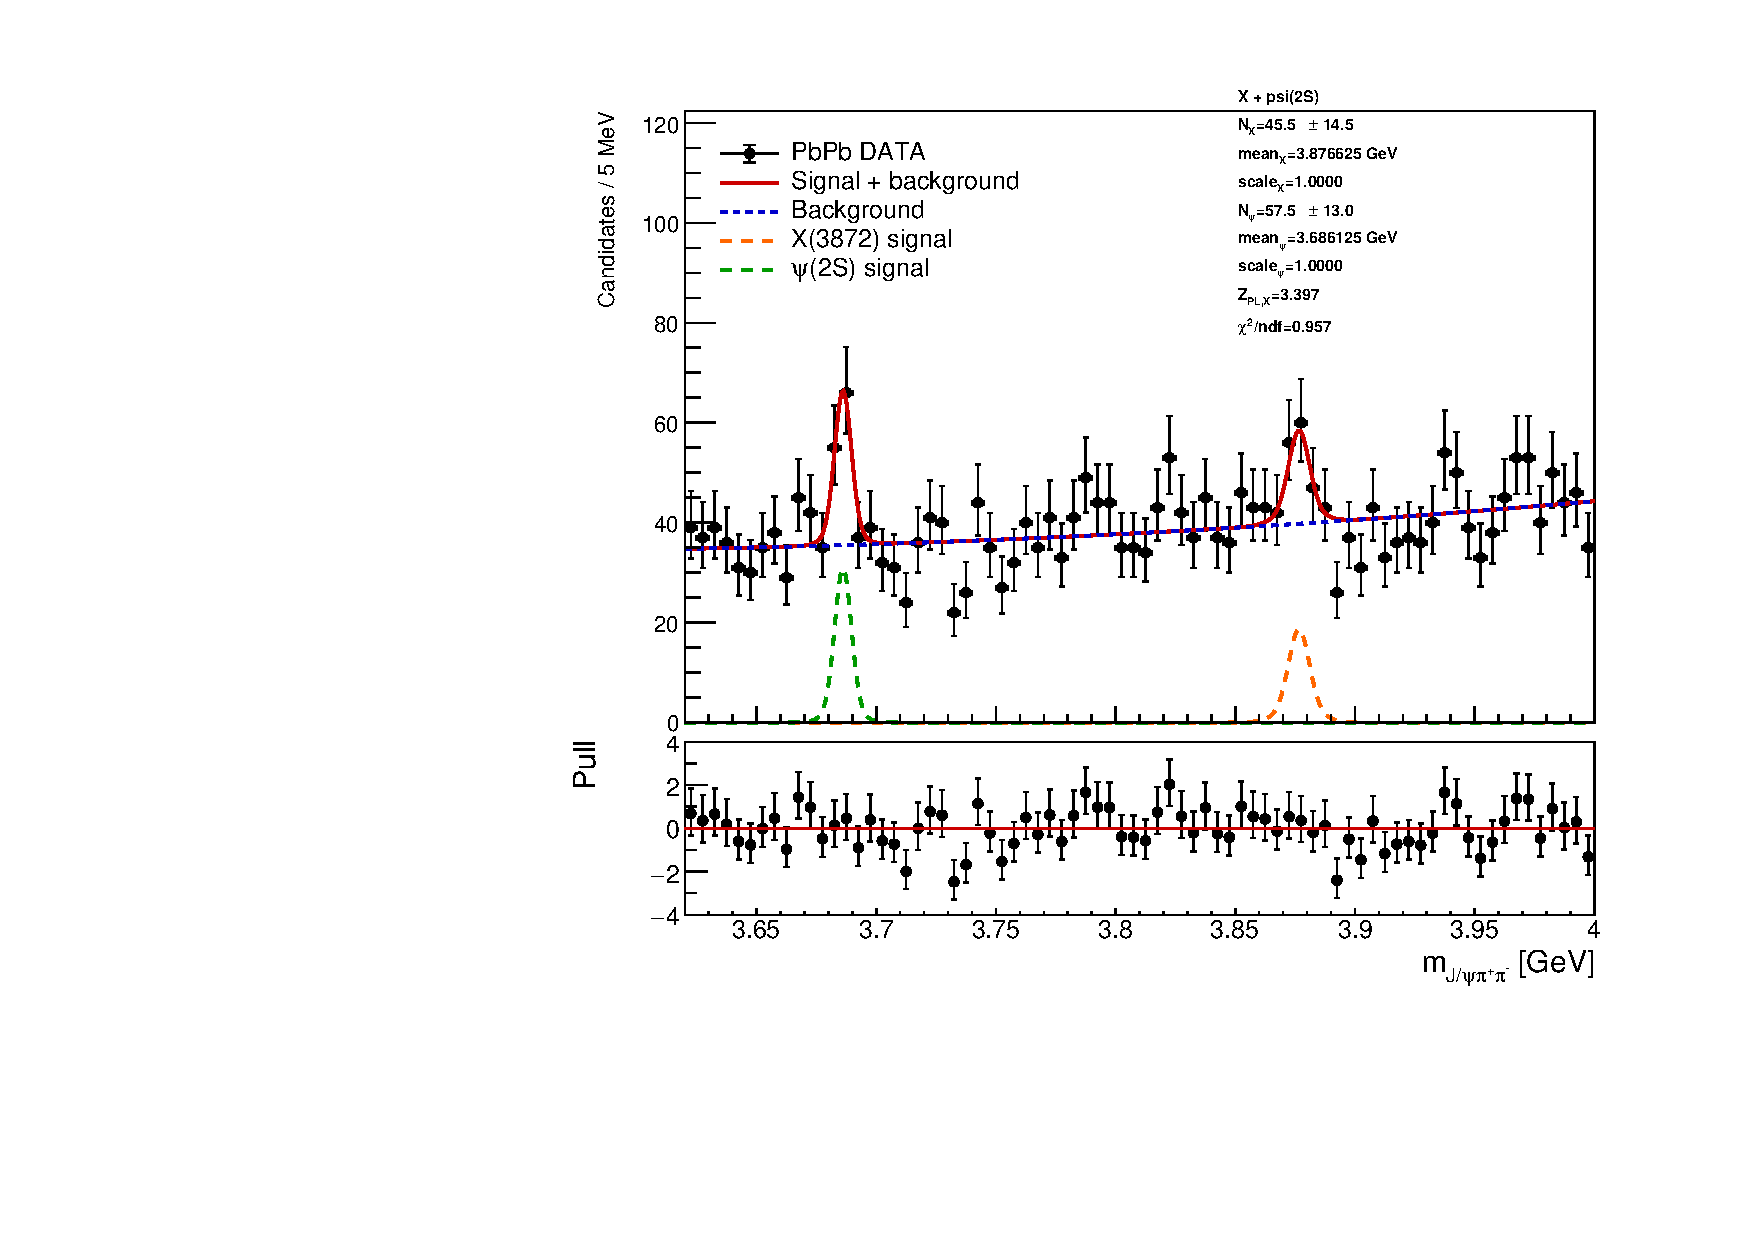
\includegraphics[width=\linewidth,height=0.72\textheight,keepaspectratio]{figures/20260920/punzi/7v17_xeff40_profile.pdf}
\column{0.33\textwidth}\small
\textbf{score $>0.890241$}\par\medskip
$N_X=45.50\pm14.53$\par
$N_{\psi(2S)}=57.51\pm13.02$\par\medskip
Same fit model as at 30\%.\par\medskip
Profile $\sqrt{q_0}=3.397$\par
\end{columns}
\takeaway{40\% is an existing reference fit, not the systematic Punzi optimum. Shown only as backup; the grid optimum remains 30\%.}
\end{frame}
